\documentclass{beamer}
\usepackage{listings}
\lstset{
%language=C,
frame=single, 
breaklines=true,
columns=fullflexible
}
\usepackage{subcaption}
\usepackage{setspace}
\usepackage{url}
\usepackage{tikz}
\usepackage{tkz-euclide} % loads  TikZ and tkz-base
%\usetkzobj{all}
\usepackage[utf8]{inputenc}
\usepackage{longtable}
\usetikzlibrary{calc,math}
\usepackage{float}

\newcommand\norm[1]{\left\lVert#1\right\rVert}
\renewcommand{\vec}[1]{\mathbf{#1}}
\usepackage[export]{adjustbox}
\usepackage[utf8]{inputenc}
\usepackage{amsmath}
\usetheme{Boadilla}
\newcommand\mytextbullet{\leavevmode%
\usebeamertemplate{itemize item}\hspace{.5em}}

\bibliographystyle{IEEEtran}

\usepackage{color}

\title{KAVACH}
\author{Automatic Train Protection System}
\institute{Indian Institute of Technology, Hyderabad.}
\date{\today}

\begin{document}


\begin{frame}
\titlepage
\end{frame}
\section{Introduction}
\begin{frame}
\frametitle{Introduction}
\begin{columns}
\column{1\textwidth}
  \begin{itemize}
  \item Automatic Train Protection (ATP) systems are designed to enhance railway safety by providing a fail-safe mechanism that ensures trains can only travel at safe speeds and maintain safe distances between each other.
  \end{itemize}
\end{columns}

\end{frame}


\section{KAVACH1}
\begin{frame}
%\frametitle{Communication Module}

\begin{figure}[h!]
  \centering
  \begin{subfigure}[b]{1\linewidth}
    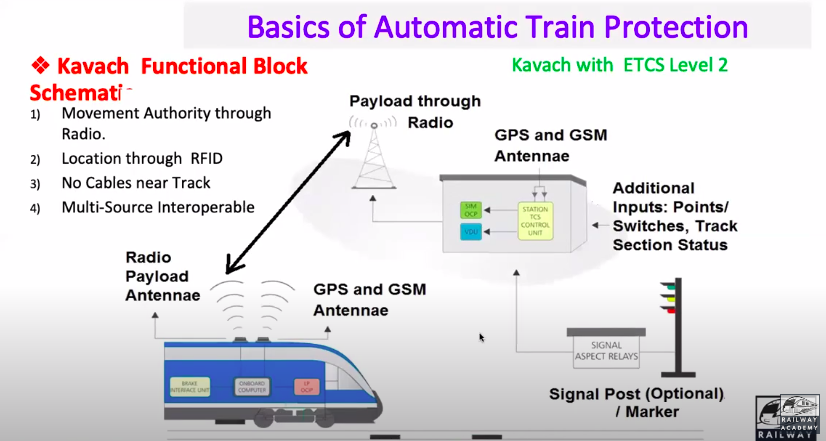
\includegraphics[width=\linewidth]{./figs/TCAS1.png}
%    \caption{Coffee.}
  \end{subfigure}

  %\caption{Broader View of communication technology with drones.}
%  \label{fig:axis}
\end{figure}

\end{frame}




\section{Data Flow}
\begin{frame}
%\frametitle{The categorization and usage of UAVs}

\begin{figure}[h!]
  \centering
  \begin{subfigure}[b]{1\linewidth}
    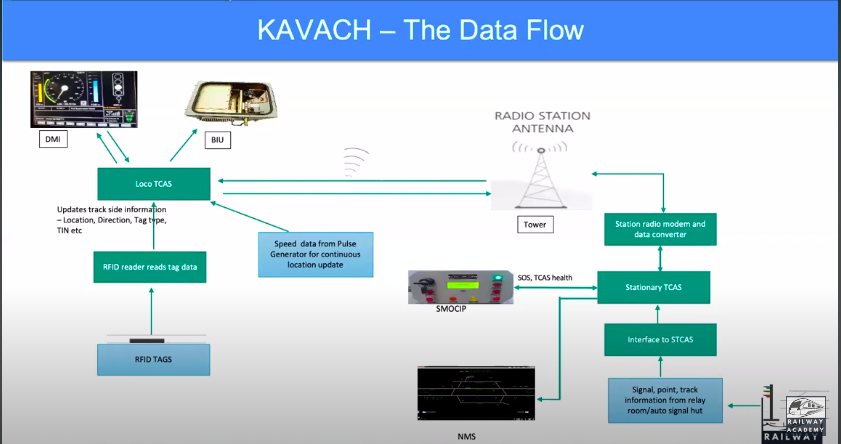
\includegraphics[width=\linewidth]{./figs/data_flow.png}
%    \caption{Coffee.}
  \end{subfigure}

 % \caption{System block diagram}
%  \label{fig:axis}
\end{figure}

\end{frame}




\section{Communication Module}
\begin{frame}
\frametitle{Need of Train protection system}
\begin{columns}
\column{1\textwidth}
  \begin{itemize}
  \item \textbf{Preventing collisions:} ATP systems can detect when a train is approaching another train or obstacle on the tracks and can automatically apply the brakes to prevent a collision.
  \item \textbf{Enhancing safety during emergencies:} In the event of an emergency, ATP systems can be used to stop the train and ensure that passengers and crew are safe.
  \item \textbf{Improving efficiency:}ATP systems can help trains run more efficiently by enabling them to travel at faster speeds without compromising safety. This can reduce travel times and increase the number of trains that can be operated on a given line.
   \item \textbf{Compliance with regulations:} Many countries require the installation of ATP systems to comply with safety regulations and ensure that trains operate within safe limits.
   
  \end{itemize}
\end{columns}

\end{frame}

\section{Basic Operations}
\begin{frame}
\frametitle{Basic Operations}
\begin{columns}
\column{1\textwidth}
  \begin{itemize}
  \item The TCAS comprises of two sub systems, namely Loco TCAS and Stationary TCAS. The communication between the Stationary TCAS and Loco TCAS is radio communication over the air.
  \item The Stationary TCAS gathers information about the current statuses of all signal aspects, Berthing Track Circuits and Point Status within the Station. Based on this information Stationary TCAS calculates the Movement Authority for each Loco within its vicinity. This information is transmitted to the Loco TCAS through Radio communication.
   \item The Loco TCAS controls its speed and supervises the train movement and other on board operations in accordance with the data received from the Stationary TCAS and section speed received through RFID tags. In the event of emergency situations, the system applies brakes thereby preventing any catastrophic accidents.
   
  \end{itemize}
\end{columns}

\end{frame}

\section{Data Flow}
\begin{frame}
%\frametitle{The categorization and usage of UAVs}

\begin{figure}[h!]
  \centering
  \begin{subfigure}[b]{1\linewidth}
    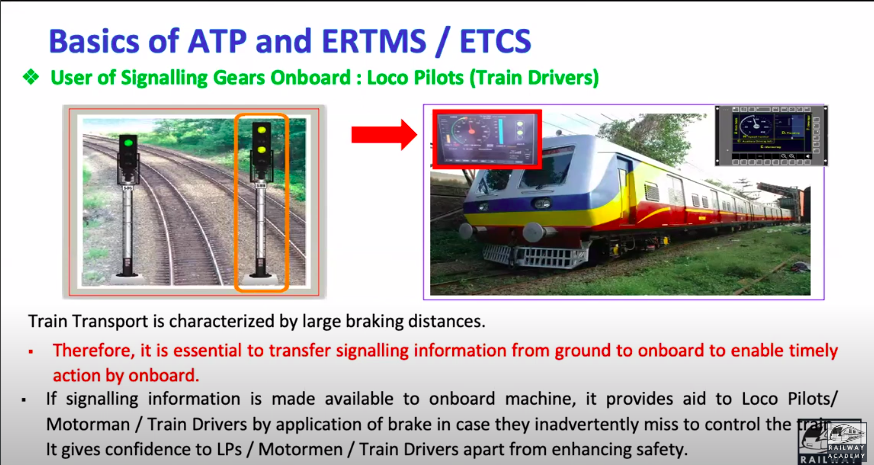
\includegraphics[width=\linewidth]{./figs/KAVACH3.png}
%    \caption{Coffee.}
  \end{subfigure}

 % \caption{System block diagram}
%  \label{fig:axis}
\end{figure}

\end{frame}

\section{Data Flow}
\begin{frame}
%\frametitle{The categorization and usage of UAVs}

\begin{figure}[h!]
  \centering
  \begin{subfigure}[b]{1\linewidth}
    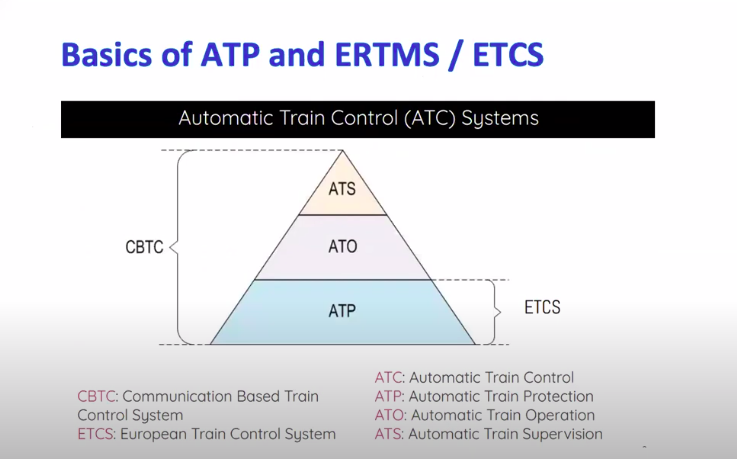
\includegraphics[width=\linewidth]{./figs/KAVACH4.png}
%    \caption{Coffee.}
  \end{subfigure}

 % \caption{System block diagram}
%  \label{fig:axis}
\end{figure}

\end{frame}

\section{Data Flow}
\begin{frame}
%\frametitle{The categorization and usage of UAVs}

\begin{figure}[h!]
  \centering
  \begin{subfigure}[b]{1\linewidth}
    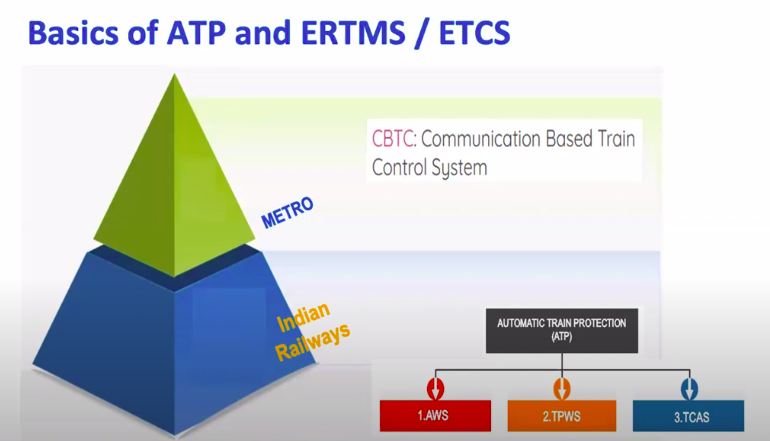
\includegraphics[width=\linewidth]{./figs/KAVACH5.png}
%    \caption{Coffee.}
  \end{subfigure}

 % \caption{System block diagram}
%  \label{fig:axis}
\end{figure}

\end{frame}

\section{Data Flow}
\begin{frame}
%\frametitle{The categorization and usage of UAVs}

\begin{figure}[h!]
  \centering
  \begin{subfigure}[b]{1\linewidth}
    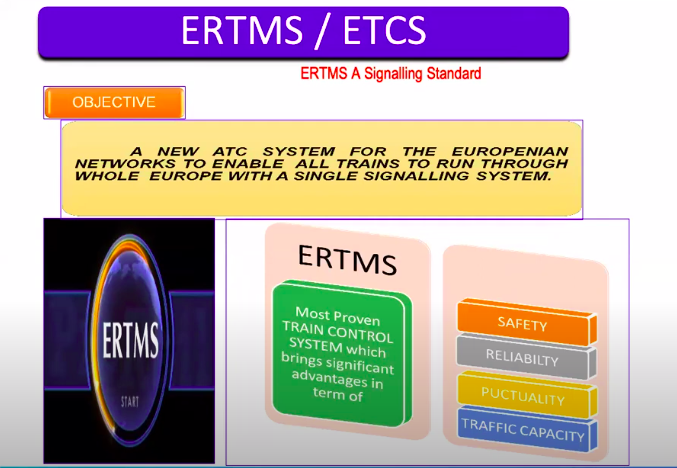
\includegraphics[width=\linewidth]{./figs/KAVACH6.png}
%    \caption{Coffee.}
  \end{subfigure}

 % \caption{System block diagram}
%  \label{fig:axis}
\end{figure}

\end{frame}

\section{Data Flow}
\begin{frame}
%\frametitle{The categorization and usage of UAVs}

\begin{figure}[h!]
  \centering
  \begin{subfigure}[b]{1\linewidth}
    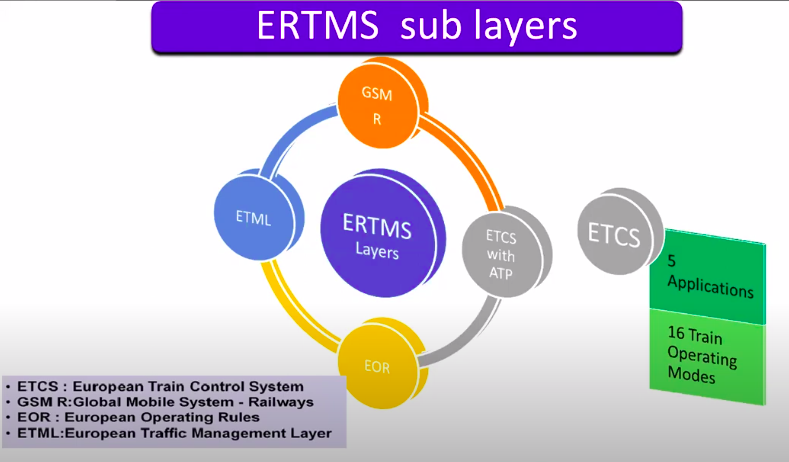
\includegraphics[width=\linewidth]{./figs/KAVACH7.png}
%    \caption{Coffee.}
  \end{subfigure}

 % \caption{System block diagram}
%  \label{fig:axis}
\end{figure}

\end{frame}

\section{Data Flow}
\begin{frame}
%\frametitle{The categorization and usage of UAVs}

\begin{figure}[h!]
  \centering
  \begin{subfigure}[b]{1\linewidth}
    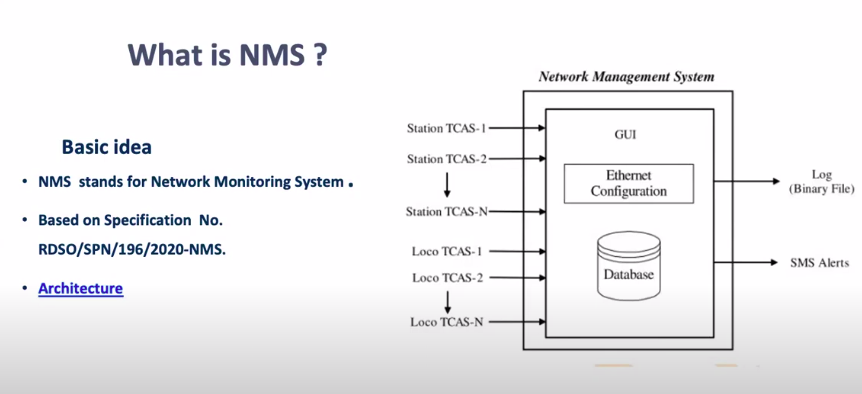
\includegraphics[width=\linewidth]{./figs/KAVACH8.png}
%    \caption{Coffee.}
  \end{subfigure}

 % \caption{System block diagram}
%  \label{fig:axis}
\end{figure}

\end{frame}


\end{document}

